The menu is opened when the palm of the left hand is facing towards the camera, and can be interacted with using the index finger of the right hand.
Unlike the other gestures-enabled commands the menu is implemented through the use of the open source project Hover UI Kit, created by Aesthetic Interactive~\citep{Hoverkit}.
The Hover UI Kit project offer three different interface modules: Hovercast, Hoverkey and Hoverpanel, where Hovercast is the one the menu is based on.
This means that several of the menu's interaction components, such as registering button clicks are handled by the Hover UI kit package.

\begin{figure}%[h!] %[H]
	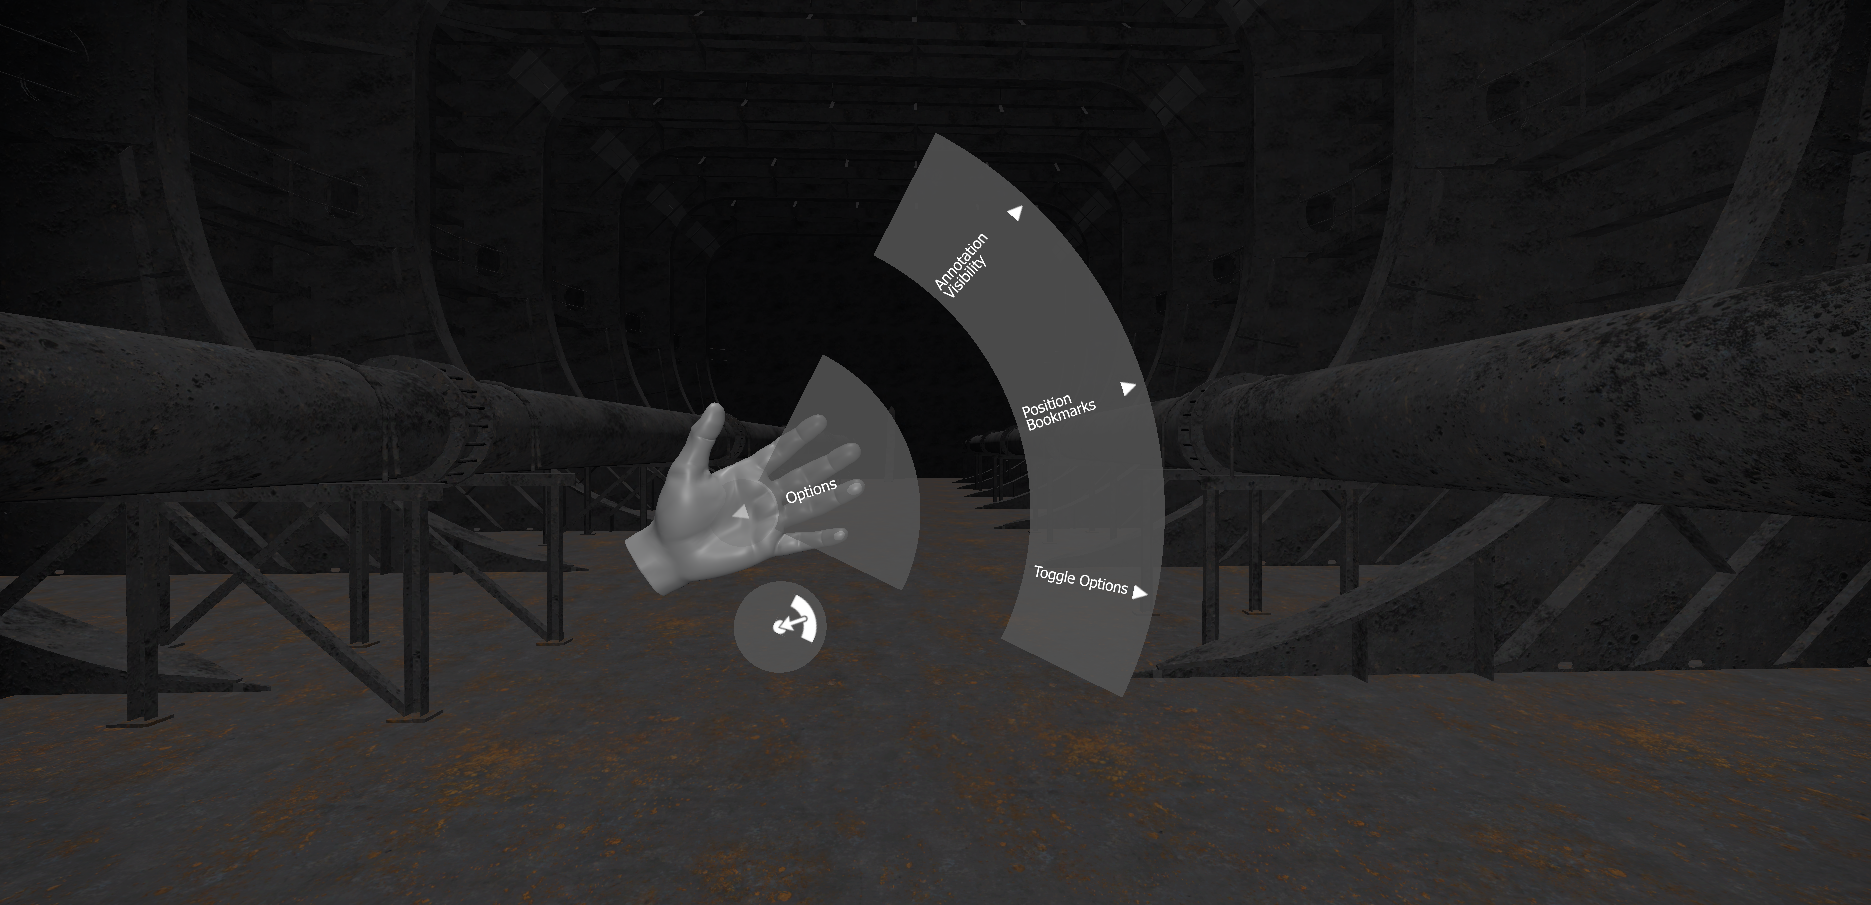
\includegraphics[width=\linewidth]{pictures/screenshots/gestures/menu_detector.png}
	\caption[The Menu]{The menu is opened when the palm of the left hand is facing towards the camera, and can be interacted with using the index finger of the right hand.}
	\label{fig:menu_detector}
\end{figure} 

The Hover UI kit main game object is present in the \texttt{GestureMenu} game object, which is a top-level game object in the project hierarchy.
\texttt{GestureMenu} has four child game object: \texttt{Hovercast}, \texttt{CursorRenderer} (which is disabled by default), \texttt{MenuHandler} and \texttt{Hoverkit}.
\texttt{Hovercast} represent the menu itself and contains the hierarchy of game objects that represents the menu buttons. 
\texttt{CursorRenderer} can optionally render a ring/cursor around the fingers that can be used as cursors.
By default only the index finger of the right hand can be used to select elements in the menu.
\texttt{MenuHandler} contains the scripts \texttt{ToggleOptions}, \texttt{Bookmarks} and \texttt{AnnotationVisibility}, which are all responsible for handling
the different actions accessable from the menu.
Lastly, the \texttt{Hoverkit} game objects contains some important "management scripts" (e.g.~\texttt{HoverItemsManager} and \texttt{HoverInteractionSettings}) related to the 
different functionality of the Hovercast menu and hoverkey keyboard in the annotation form (more on that later). The \texttt{Hoverkit} game object also
contains a Cursor game object, which contains a hierarchy with representations of the left- and right hand, and then each hand's respective finger objects. 
In this object hierarchy we can select which fingers that are cursors, which hand that can "host" or "spawn" the menu etc. As mentioned earlier
the default setting is that the menu only can be created by the left hand palm and only interacted with using the right hand index finger. 
 
\subsection{The Menu Objects}
The \texttt{Hovercast} game object has four game objects as direct children, which all represent a visible part of the hovercast menu:
\texttt{OpenItem}, \texttt{TitleItem}, \texttt{BackItem} and \texttt{Rows}. 

\begin{figure}%[h!] %[H]
	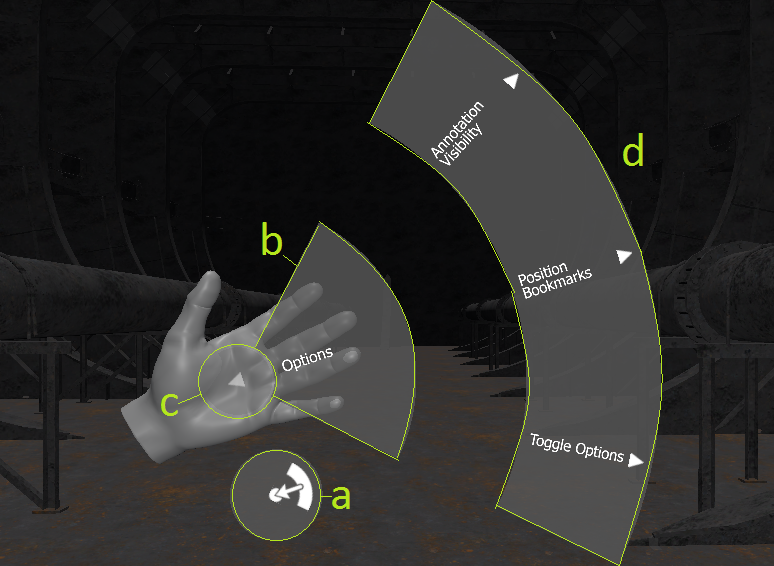
\includegraphics[width=\linewidth]{pictures/screenshots/menu/menu_components.png}
	\caption[The Menu components]{The main menu object is represented with four sub-objects: \texttt{OpenItem} (a), \texttt{TitleItem} (b), \texttt{BackItem} (c) 
			 and \texttt{Rows} (d).}
	\label{fig:menu_components}
\end{figure}

While the \texttt{OpenItem}, \texttt{TitleItem} and \texttt{BackItem} uses functionality that is the default in Hover UI Kit, and is readily available in presets,
\texttt{Rows} contains quite a bit of implementation specific objects. The term "row" will her refer to a set of one or more buttons, which are clickable and visible at together,
in the "row section" of the menu (see~\vref{fig:menu_components} (d)). The \texttt{Rows} game object has four direct children: \texttt{Root}, \texttt{RowA}, \texttt{RowB} 
and \texttt{RowC}. \texttt{Root} is the root menu row, i.e the row that is visible when the menu is opened, and contains three buttons, each represented as 
child game objects of \texttt{Root}: \texttt{ItemA}, \texttt{ItemB} and \texttt{ItemC}. Each of these buttons leads to their own submenu, i.e their own row. 
\texttt{ItemA} represent the "Annotation Visibility" submenu, and brings up \texttt{RowA} as the "current row" instead of root when clicked. \texttt{ItemB} ("Position Bookmarks") 
and \texttt{ItemC} ("Toggle Options") follows the same logic and lead to \texttt{RowB} and \texttt{RowC} respectively (see~\vref{table:menu_hierarchy} for the hierarchical overview. 
This transition is handled by the \texttt{HovercastRowSwitchingInfo} component that is attached to each button game object.  

\renewcommand{\DTstyle}{\textrm\expandafter\raisebox{-0.7ex}}
\DTsetlength{1em}{1em}{0.2em}{0.4pt}{0.4pt}
\setlength{\DTbaselineskip}{2\baselineskip}

\begin{table}[]
\label{table:menu_hierarchy}
	\dirtree{%
	.1 Root menu.
	.2 Annotation Visibility (submenu/row).
	.3 Always visible (radio button).
	.3 Visible with LOS (radio button).
	.3 Invisible (radio button).
	.3 Use Glow (checkbox).
	.3 Back (button).
	.2 Position Bookmarks (submenu/row).
	.3 Origin (button).
	.3 Back (button).
	.2 Toggle Options (submenu/row).
	.3 Toggle crosshair (button).
	.3 Enable gestures/Disable gestures (button).
	.3 Combined XYZ gestures/Distinguish XYZ gestures (button).
	.3 Back (button).
	}
\caption[The Menu Hierarchy]{The Menu Hierarchy}
\end{table}

\texttt{RowA}, \texttt{RowB} and \texttt{RowC} each contains game objects that represents buttons in that submenu. 
In these button game objects \texttt{HoverItemDataSelector}, \texttt{HoverItemDataRadio} or \texttt{HoverItemDataCheckbox}, for "regular buttons", radio buttons and 
checkboxes respectively, are attached as components. These components are all either directly or indirectly subclasses of \texttt{HoverItemDataSelectable}, which 
contains important properties like "Label" (i.e the button text value) and a list of eventhandler. An example of this is \texttt{ItemCB} in \texttt{RowC}, which has 
the label "Disable Gestures" and has an entry in the "OnSelectedEvent" list. This entry is a reference to the \texttt{GestureOptions} class' function \texttt{toggleGestures}. 

\subsection{The MenuHandler Scripts}
The menu makes use of three scripts to handle all actions: \texttt{AnnotationVisibility}, \texttt{Bookmarks} and \texttt{GestureOptions}.
These are all components of the \texttt{MenuHandler} game object and serve their seperate submenus (i.e Row A, B and C) and buttons. 

The \texttt{AnnotationVisibility} script's main purpose is to interact with the active camera rig's annotation camera, and manipulate the way
the annotations are presented to the user. This include choosing between three annotation presentation modes: "Always visible", "Visible with LOS" and 
"Invisible", and choosing whether to use a glow effect on annotation or not. This is done by manipulating the active annotation camera's culling mask 
and clear flags using bit shift:

\begin{table}
\label{table:annotation_visibility_code}
\lstset{style=csharp}
\begin{lstlisting}
public void alwaysShow()
{
	//Include the SphereAnnotation layer to the culling mask and use "Depth only" as clear flag.
	annotationCamera.cullingMask |= 1 << LayerMask.NameToLayer("SphereAnnotation");
	annotationCamera.clearFlags = CameraClearFlags.Depth;
}

public void showWithLOS()
{
	//Include the SphereAnnotation layer to the culling mask and dont clear anything.
	annotationCamera.cullingMask |= 1 << LayerMask.NameToLayer("SphereAnnotation");
	annotationCamera.clearFlags = CameraClearFlags.Nothing;
}

public void hide()
{
	//Only render objects in the first layer (Default layer)
	annotationCamera.cullingMask &= ~(1 << LayerMask.NameToLayer("SphereAnnotation"));
}
\end{lstlisting}
\caption[Annotation visibility manipulation]{Annotation visibility manipulation example in C\# code. This code snippets makes use of 
		bit shifts on the annotation camera's culling mask and clear-flags properties.} 
\end{table}

The functional differences between the annotation presentation mode with or without glow are covered in~\vref{sec:annotations}. 

The \texttt{Bookmarks} script's main purpose is to handle what in the menu is refered to as "Positional bookmarks". The primary idea behind positional bookmarks 
is to allow the user to save specific points of interest in the model to be able to quickly return there, just like one could bookmark a web page in a web browser. 
In the current iteration of the application it isn't possible to create new bookmarks, so the only available one is the "Origin" bookmark, which is the position and orientation
the user has when first entering the application (useful to reset the position e.g.~ if the user should get lost in some way). In the script this functionality is accomplished
by having a linked list of transforms (a unity game object component storing relevant information) and a referance to the \texttt{MasterController} game object. 
The \texttt{MasterController}'s position and rotation in the applications first rendered frame is stored as the first entry in this list and, should the user click the 
appropriate menu button "Origin", in the "Positional bookmarks" submenu, the function \texttt{GoToBookmark(int index)} should be called with index = 0 as index argument. 
The \texttt{GoToBookmark} function then looks up the transform stored at index \textit{i}, and if successful sets the position and orientation coordinates of the 
\texttt{MasterController}'s transform. The user will experience this as the camera "teleporting" to the same spot as the player started on when entering the 3D model.

The \texttt{GestureOptions} script's main purpose is to handle options related to gestures, and handles two menu elements from the Toggle Options submenu:
"Enable gestures" / "Disable gestures" (one button with a context dependent label) and "Combine XYZ gestures" / "Distingush XYZ gestures" (also context dependent label). This is 
primarily done by two of its functions \texttt{toggleGesturesActive} and \texttt{toggleGestureMode}, which both use the context dependent toggle principle 
and functions in the \texttt{GestureHand} class. In the implementation a toggle is simply to swap to the opposite value of the current, with two possible values available (i.e 
toggle + true = false and toggle + false = true).


\texttt{toggleGesturesActive} checks the value of the instance variable \texttt{GesturesEnabled} 
and either disables or enables gestures based on what is variable holds. If \texttt{GesturesEnabled = true}, i.e that gestures are enabled, the function 
disables gestures by calling each \texttt{GestureHand}'s \texttt{disableDetectors} function, swaps hand materials to the "disabled-material" and swaps the 
\texttt{GesturesEnabled} variable to its opposite value (i.e now \texttt{GesturesEnabled = false}). In the opposite case, i.e when the function is called and 
the \texttt{GesturesEnabled} variable has the value false, gestures are enabled by calling each \texttt{GestureHand}'s \texttt{enableDetectors} function, swapping
hand materials to the "none-material" and swapping the \texttt{GesturesEnabled} variable to its opposite value (i.e now \texttt{GesturesEnabled = true}). 

\begin{table}
\label{table:gesture_options_code}
\lstset{style=csharp}
\begin{lstlisting}
public GestureHand[] hands;
private static bool gesturesEnabled;

public void toggleGesturesActive(HoverItemDataSelector selector)
{
	if (gesturesEnabled)
	{
		selector.Label = "Enable Gestures";
		foreach (GestureHand hand in hands)
		{
			hand.disableDetectors();
			hand.ToggleHandMaterial(hand.handMaterials[7]);
		}

	}
	else
	{
		selector.Label = "Disable Gestures";
		foreach (GestureHand hand in hands)
		{
			hand.enableDetectors();
			hand.ToggleHandMaterial(hand.handMaterials[0]);
		}
	}

	gesturesEnabled = !gesturesEnabled;
}
\end{lstlisting}
\caption[The GestureOptions class]{The GestureOptions class can be called to enable or disable all detectors based on its current state.} 
\end{table}

The \texttt{toggleGestureMode} functions in a very similar manner as \texttt{toggleGesturesActive} and uses a boolean value present in the \texttt{GestureHand} instances
to toggle between a combined or separate state for movement gesture (i.e whether to have movement gestures in the x, y and z plans combined or separate.  